\chapter{Results}
\label{sec:results}

In the current chapter, results of GAT-Denoiser are presented.
Further, some interesting findings are illustrated and GAT-Denoiser
is compared to U-Net and BM3D\cite{bm3d}.


\section{Dataset}
GAT-Denoiser is tested on lodopab-ct dataset \cite{lodopab-dataset}, which is a 
benchmark dataset for low-dose ct reconstruction methods and therefore well suited for our domain.

The dataset consists of 35820 train images and 3553 test images.
All these images are having resolution 64.

\begin{figure}[H]
  \centering
  \hfill
  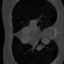
\includegraphics[width=0.2\textwidth]{ct_im_0.png}
  \hfill
  
\includegraphics[width=0.2\textwidth]{ct_im_1.png}
  \hfill
  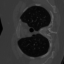
\includegraphics[width=0.2\textwidth]{ct_im_2.png}
  \hfill
  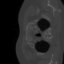
\includegraphics[width=0.2\textwidth]{ct_im_3.png}
  \hfill
  \caption{Some train images of lodopab-ct dataset.}
\end{figure}



\section{Training setup}
Training of GAT-Denoiser has been done on the HPC-cluster scicore of the University of Basel.
During training, up to 4 titanx GPUs with 12 GB RAM have been used.


\section{Source code}
Source code of the project is available on GitHub\footnote{https://github.com/cedricmendelin/master-thesis}.

\subsection{Python packages}
The following important python packages have been:


\section{Small Experiments}
Some small experiments to find best suited architecture for GAT-Denoiser.
\begin{itemize}
  \item 1024 train images
  \item 100 validation images
\end{itemize}

Test many different settings:
\begin{itemize}
  \item K-nn size ([2,4,6,8,10,12]) and sampling points / Graph feature dimension (512, 1024, 1536, 2048)
 
  \item GAT architecute (Layers, Heads, Loss FBP, Fixed conv)
  \item Convolution (with, without, multiple channels)
  \item Loss Sino and FBP
  \item U-Net with and without
  \item Different SNR levels
  \item Learning over SNR range? (slighly not)
  
  
\end{itemize}


\section{Complete Experiments}
Use complete set of experiment dataset.

Compare with :
\begin{itemize}
  \item Only FBP
  \item FBP  + U-Net
  \item FBP  + Bm3d
  \item bm3d on sino + FBP
  \item Evantually same with non-local means
\end{itemize}
Compare with Bm3d (applied to noisy sinogram, after FBP and after FBP + Unet)

